%
% einleitung.tex -- Beispiel-File für die Einleitung
%
% (c) 2020 Prof Dr Andreas Müller, Hochschule Rapperswil
%
% !TEX root = ../../buch.tex
% !TEX encoding = UTF-8
%
\subsection{Kartesisch\label{geodaeten:section:Linienelemente:Kartesisch}}
Wie in Abbildung \ref{geodaeten:figure:Linienelemente:Kartesisch:figure1} zu sehen ist kann ein Wegstück auf einer Kurve im zweidimensionalen kartesischen Raum mit
\begin{equation}
	\Delta s \approx \sqrt{\Delta x^2 + \Delta y^2}
\end{equation}
approximiert werden.
Durch Verkleinerung der Wegstücke bis zum Infinitesimal 
\begin{equation}
	d s = \sqrt{d x^2 + d y^2}
\end{equation}
kann das Linienelement aufgestellt werden als\footnote{
Betrachtet man die Masseinheiten, erkennt man dass sie mit $ds^2 = dx^2 + dy^2 = \left( \frac{dx^2}{dt^2}+\frac{dy^2}{dt^2} \right) \cdot dt^2 \Leftrightarrow \text{Länge}^2 = \text{Geschwindigkeit}^2 \cdot \text{Zeit}^2$ auch aufgeht.
}
\index{Linienelement!kartesisch}%
\begin{equation}
 	ds^2 = d x^2 + d y^2.
 	%\left(\dot{x}^2 +\dot{y}^2\right) %\cdot dt^2 .
 	\label{geodaeten:equation:Linienelemente:Kartesisch:equation1}
\end{equation}

\begin{figure}
	\centering
	
	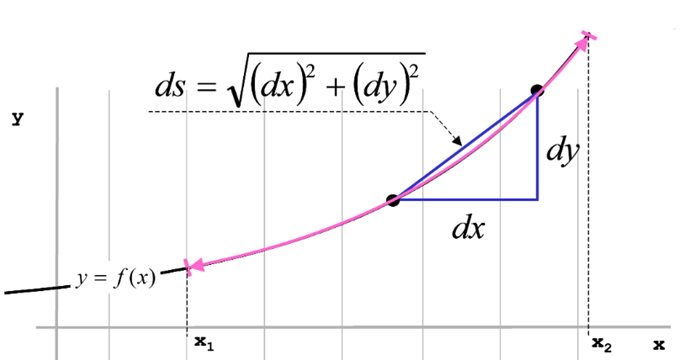
\includegraphics[width=0.7\linewidth]{papers/geodaeten/Abbildungen/Linienelemente/LinKartes1}
	\caption{Linienelement im Kartesischen Raum. Bildquelle: \cite{geodaeten:kartesisch}} 
	\label{geodaeten:figure:Linienelemente:Kartesisch:figure1}	
\end{figure}
